\chapter{Design and Implementation} \label{chap:impl}

The primary deliverable of this dissertation is a system (shown in Figure \ref{fig:overview}) that is able to generate metabolic models of cell-free systems.
Our system has four major parts.
First, we ingest experimental data and incorporate it into a standardized format.
Next, we convert the data into a group of cellular metabolic models and sample fluxes from those models to create a dataset.
Then, we perform dimensionality reduction to elucidate underlying trends in the experimental data.
Finally, we use those insights to reduce the original, overspecified models to standalone cell-free metabolic models.

\section{Data gathering}
In order to build a robust model that reflected biological reality, we first had to generate the data we wanted to use for training.
Gathering high quality biological data is difficult and was crucial key to the success of the system as a whole.
We describe the high level process of creating a cell-free system and running the experiments below.
The full experimental protocol can be found at dx.doi.org/10.17504/protocols.io.kz2cx8e.

\subsection{Cell-free systems}
As shown in Fig \ref{fig:cfps}, creating a cell-free protein expression system involves three main steps: growing and lysing cells, supplementing with energy substrates, and adding custom \gls{dna} constructs.
Our protocol is based off of the open protocol out of the Federici lab \cite{medina2017cfps}.
We begin by growing up 1L of BL21 \ecoli cells in an overnight culture of \gls{lb} until they have reached \gls{od} of 1.6.
Then, we spin down the cells and remove the supernatant, storing the pellet in the refrigerator overnight if necessary.
Next, we perform 3 more sets of spins and washes with S30 buffers to remove any extracellular debris.
Finally, we use a bead beater to lyse the cells and spin one last time to remove the cellular debris and beads.
At the end of this process we have cell extract which can be stored in a -80\degree freezer.
\begin{figure}[t!]
\begin{center}
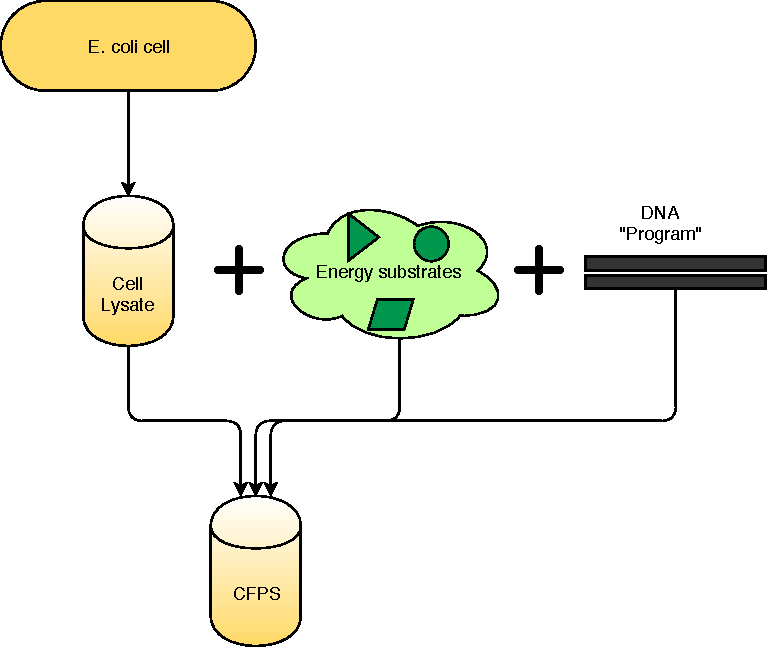
\includegraphics{figs/CellFreeSetup.pdf}
\caption{Overall process for creating a \gls{cfps}}
\end{center}
\label{fig:cfps}
\end{figure}

Once we have this cell extract, we have the core cellular machinery that is necessary for transcription and translation.
However, we need to add the cofactors and reactants that are important for the transcription and translation reactions.
So, we add energy substrates to the cell extract to create a cell-free protein expression system.
These substrates include energy substrates such as \gls{camp}, maltodextrin, and \gls{nad}.
They also include vital parts of transcription and translation such as \glspl{ntp}, \glspl{aa}, and \glspl{trna}.
See Table \ref{tab:cf-nrg} for a complete listing of the reactants and their purpose in the system.
Table \ref{tab:cf-conc} shows the final concentration for each substrate.

%TODO FIX TABLES

\begin{table}[]
\centering
\caption{List of reactants for a 50 \gls{ul} \gls{cfps} reaction. 
Note that MDX is a mixture of substrates (see the complete list in \ref{tab:cf-conc}.
\glspl{aa} includes all 20 of the amino acids.}
\label{tab:cf-nrg}
\begin{tabular}{lll}
Reactant     & Amount (\gls{ul}) & Purpose                         \\
MDX          & 5               & Energy substrates               \\
\glspl{aa}          & 10              & Building blocks for translation \\
\gls{peg}          & 2.5             & Molecular crowding              \\
\gls{hmp}          & 1               & Phosphate source                \\
\gls{mg}           & 0.74            & Important cofactor              \\
\gls{k}            & 0.8             & Charge homeostasis              \\
\gls{dna}          & 0.8             & Template for protein production  \\
Cell Extract & 25              & \gls{tx}/\gls{tl} machinery                 \\ \hline
\gls{cfps}         & 50              & Protein production             
\end{tabular}
\end{table}

Given this cell-free expression system, we have essentially assembled a biological computer.
Whatever \gls{dna} "program" is added, the system will work to produce the appropriate protein result.
This platform is incredibly powerful because it allows us to easily insert these \gls{dna} programs and see results within a few hours.
A typical biological timeline would take far longer because living cells would have to be coerced to uptake the \gls{dna} and incorporate it into their production process.

%TODO talk about debugging/contamination issue

\subsection{Datasets}
We used the protocol above to create two datasets for training.
The first dataset was created by hand and followed standard lab procedures.
We pipetted each of the reactants in the ratios specified by Table \ref{tab:cf-nrg} to create a 200 \gls{ul} mastermix. 
From that mastermix, we then used 5 \gls{ul} aliquots combined with each of our different reaction conditions.
In order to test different reaction conditions, we added an additional 1 \gls{ul} of various reactants.
For this dataset, we experimented by adding 16 differing ratios of sugar, phosphate, potassium, and nucleotides.
The \gls{dna} circuit in the \gls{cfps} system simply produces \gls{rfp}, so we were able to judge the amount of protein production by measuring fluorescence readout with a plate reader.

However, there are multiple downsides to doing this by hand, so our second dataset was created using a Labcyte Echo acoustic liquid handler.
Creating large datasets by hand takes a long time and limits the amount of data one can generate.
Additionally, pipetting by hand has an intrinsic error, so we hoped that automating the creation of the reactions would reduce human error.
The Echo is an acoustic liquid handler that can combine different amounts of liquid to create each of the \gls{cfps} reactions.
We were able to perform the experiments at 2\gls{ul} of \gls{cfps} system and 500 \gls{nl} of additional reactants.
The use of automation allowed us to test 48 different reaction conditions and shows that this could be grown to an even larger scale.

Finally, we received a third dataset from the recent Karim and Jewett paper that uses \gls{cfps} systems to perform metabolic engineering~\cite{karim2018controlling}.
Our protocol is very similar to the one used in the Jewett lab, though some of the reactant concentrations differ.
This dataset is primarily useful because it was created in a different lab and they investigated a metabolic pathway whose output is not fluorescence.
Since it was created in different lab conditions, we can check that our model is learning something about cell-free systems in general, not just overfitting our data.
The pathway that they investigated is an inherently metabolic pathway, so we can see if our metabolic model is better able to describe these types of gene circuits.

\section{Data ingestion and incorporation}

\subsection{Data ingestion}
Since this system is intended to aid biologists in their experiments, we wanted to make it end-to-end and as easy to use as possible.
With that in mind, we created tools to automatically incorporate the experimental setup into the models.
Figure \ref{fig:ingest} shows the two main ways that the experimental setup could show up.
The first is in the form of end concentrations of the different reactants in the cell-free system.
This is the easiest because in that case we can simply convert concentrations into fluxes.
Fluxes have the unit mol/min/gDW, so we can convert metabolite concentrations into flues using the following equation from MetaboTools~\cite{aurich2016metabotools}:
\begin{equation}
f = \frac{m}{c * t * 1000.0}
\end{equation}
where $f$ is the flux value, $m$ is the concentration of our metabolite, and $c$ is the overall concentration of the cell.
We set t to be 24, the time scale of our reactions.
Using this equation our tool is able to ingest a \gls{csv} mapping the name of the reactant to the final concentration and turn them into flux constraints.

However, we also support users who might only know the relative amounts of each reactant that they are adding.
This is important because many biologists may have a protocol that they follow that tells them how to make a \gls{cfps} system, but they may not know the concentrations in their mixture.
To support these users, we allow them to upload a \gls{csv} (or combination of \glspl{csv}) that contains information about each reactant used to make the system.
For each reactant, we require name of each reactant, the molecular weight, the volume used to create the stock, the weight used to create the stock, and the final volume added to the cell-free reaction.
We parse this information to calculate the final concentration of each reactant in the \gls{cfps} system.
Once we have manipulated the data into the same form as the first type of upload, we can proceed with the rest of our computational pipeline.

\begin{figure}[t!]
\begin{center}
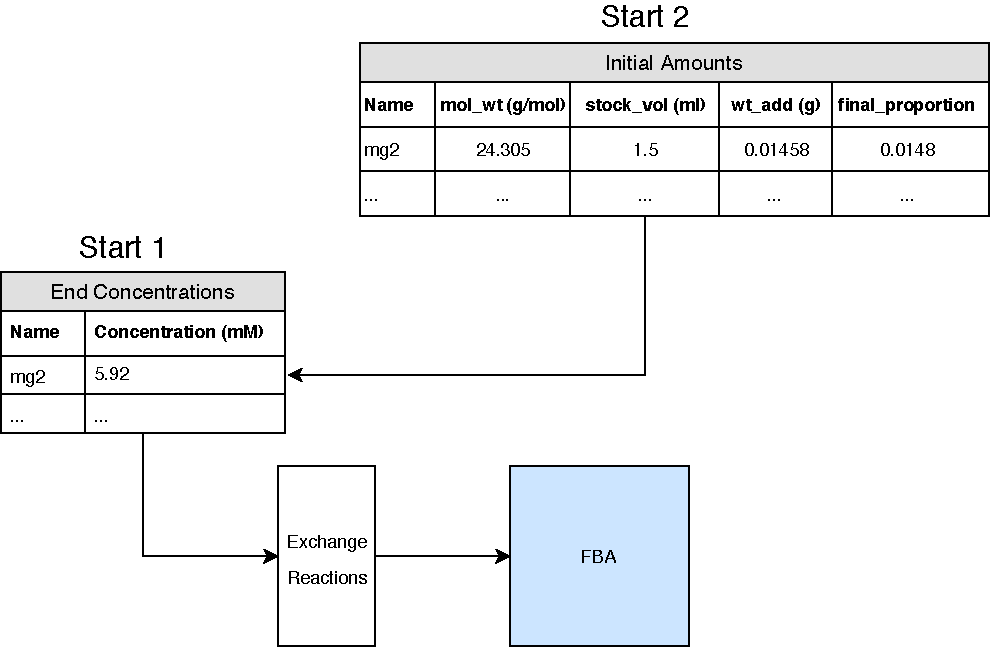
\includegraphics{figs/DataIngestion.pdf}
\caption{Two possible ways to incorporate the experimental setup in our pipeline.
In Start 1, the user already knows the final concentrations of each reactant and can upload that as a \gls{csv}.
Otherwise, the user can upload information about the reactants that are added and our tools will automatically calculate the final concnetrations of each reactant.}
\end{center}
\label{fig:ingest}
\end{figure}

\subsection{Data Incorporation} \label{sec:incorp}
After we ingest the experimental setup, we need to incorporate it into our \gls{fba} model.
We use the \gls{cobra}py python package~\cite{ebrahim2013cobrapy} to handle our \gls{fba} models.
The base model that we start with is the iJO1366 model for \ecoli which consists of 1805 metabolites and 2583 reactions~\cite{orth2011comprehensive}.
This model needs to be adapted to cell-free systems because they no longer have the same physical structure as \ecoli cells.
First, we need to make the cell-free reaction reflect the fact that there are no longer any membranes or cellular compartments.
We do this by iterating over every reaction that contains a periplasmic or extracellular component.
For each reaction, we then replace every metabolite with either the corresponding cytosolic metabolite or, if no corresponding metabolite exists, we just change the metabolite to be in the cytosol.
At this point, we have all of the reactions occurring in the same location, which reflects how a \gls{cfps} system works.

Our next task is to handle how exchange reactions are dealt with in the model.
Exchange reactions are pseudo-reactions that allow us to constraint the amount of a reactant that is allowed to be in the model.
For each of the reactants in our \gls{cfps} system, we replace the bounds on the exchange reactions based on the fluxes we calculated from the setup data earlier.
At the end of this process, we have converted the full-scale \ecoli model to better approximate a \gls{cfps} system.
%TODO claim more credit
While still overspecified, we have now created a new base cell-free model.

We also extend this model to explicitly incorporate the transcription and translation reactions that are so crucial to \gls{cfps} systems.
Most \gls{fba} models do not explicitly consider the transcription and translation reactions.
However, earlier work from the Varner lab incorporated these reactions into a \gls{fba} model specifically to try to model a cell-free system~\cite{vilkhovoy2017sequence}.
This earlier work created the \gls{fba} model by hand and is written in Julia.
We built helper tools such that, given the sequence of the gene of interest, we can automatically generate a version of the Varner model.
Next, we convert that model to Python and extract the relevant transcription and translation reactions.
We incorporate those reactions into our model and then can set the production of the protein of interest as our \gls{fba} objective.
This model is called our TXTL cell-free model.

%As a linear programming problem, we also need to set a custom objective to optimize for.
%Usually this is the biomass objective, which encapsulates everything necessary for bacterial growth.
%However, since we don't care about growth, just production, we can use our own objectives.
%For us, the typical objective will be the production of some protein since that's the purpose of the \gls{cfps}.

\section{Dataset generation}

\subsection{Model generation}
Once we have created these base models, we can use them in conjunction with the different experimental conditions to create a different model for each condition.
To do this, we take in a \gls{csv} consisting of the experimental conditions and a quantitative output.
Each row represents a different experiment.
The columns contain either the different concentrations for starting reactants or the different amounts added.
In the latter case, we can re-calculate the final concentrations of each of the reactants for each experimental starting condition.
In both cases, once we have the new final concentrations for each reactant, we create a new \gls{fba} model.

Were we simply to solve the different models we have created, many would have the same flux results.
For these naive models, Section \ref{sec:cmp} shows that they do not describe our biological results very well.
Clearly, \gls{fba} alone cannot describe the full richness of a real system.
We also have the problem that the model is overspecified.
These \gls{fba} models contain every reaction that is occurring in a steady state bacterium
While we do harvest the bacteria at steady state, some enzymes will degrade and others will not be as important in cell-free systems.
These types of changes cannot be encapsulated solely through a change of objective function and changing to a single-compartment reaction.

One can imagine \gls{fba} as a coarse bijective function, so points that vary only slightly in the input space will get projected into the same output point.
We want to do better by first passing the fluxes through a dimensionality reduction technique such as a \gls{vae}.
However, in order to do this, we first need a large dataset of fluxes to train on.
Since we only have a small number (dozens, not hundreds) of models, we cannot simply use the fluxes from the optimal solution to the model.
We supplement our dataset by flux sampling from each model.

\subsection{Flux sampling}
Flux sampling is the process of sampling possible fluxes through each reaction.
This gives us a distribution of fluxes for each reaction, for each model.
We use optGpSampler to sample 2000 fluxes from each of our models~\cite{megchelenbrink2014optgpsampler}.
Figure \ref{fig:fl-samps} shows what happens as we increase the number of samples we draw from each model.
Clearly, we can see that increasing the number of samples leads to a more normal distribution.

%TODO: Insert figure

Each model has different experimental conditions and therefore has slightly different flux distributions for each reaction.
So, after we generate flux samples for each model, we can combine the sampled fluxes to generate two new datasets.
One dataset is flat---meaning we simply concatenate all of the sampled fluxes into a dataset of size $2000E x R$ where $E$ is the number of experiments and $R$ is the number of reactions.
This dataset is useful to investigate the fluxes and see if we can perform dimensionality reduction to gain insights on the fluxes in our models in general.
The other dataset we can make involves sampling with replacement from the fluxes of each model and then stacking the fluxes to create a new dataset.
This dataset has size $N x E x R$ where N is the number of samples with replacement we drew.
Using this dataset allows us to incorporate the correlation term in our \gls{vae}.

\section{\gls{vae}}
The key part of our system was the usage of a Variational Autoencoder in order to reduce the dimensionality of our model.
Our \gls{vae} was implemented using the Keras framework~\cite{chollet2015keras} and the implementation was designed to be as modular as possible.
We wanted to make the \gls{vae} as modular as possible so that end-users would be able to easily change the parameters of the \gls{vae} without having to have any prior training in deep learning.
%TODO: explain why this is easier for people to use
Thus, our implementation is able to take in either a flat or stacked dataset, a list of layer sizes, the number of latent dimensions, how to scale the inputs, and whether or not to use the custom correlation loss function.

The structure of the \glspl{vae} we used are as follows.
We experimented with two different layer structures, a 2-layer \gls{vae} with layer sizes 1024 and 256 and a 3-layer \gls{vae} with layer sizes 1024, 512, and 256.
We also tried using latent dimensions of size 2 and 10.
For activations between layers of the encoder and the decoder, we used \gls{relu} activations~\cite{nair2010rectified}.
The activation of our final layer of the decoder is one of sigmoidal, tanh, or linear, depending on how the dataset was scaled.
When using the custom correlation loss function, we required a stacked dataset, otherwise a flat dataset could be used.

\subsection{Correlated \gls{vae}}
The key insight for the correlation loss is that we did not just want to reduce our dimensionality in an unbiased way---we care about how well it describes real-world data.
Thus, we can use our additional information to perturb the latent space to better reflect biological reality.
We know what the relative rankings of the different models should be, so we can add a correlation loss term between the experimental data and the latent representation.
Recall Equation \ref{eqn:vae-loss} that described the \gls{vae} loss function.
We now train with a modified loss function:

%TODO explain why

\begin{equation}\label{eqn:corr-loss}
\mathcal{L}(\theta, \phi) = - E[\log p_{\theta}(x_i | z)] + KL(q_{\phi}(z | x_i) || p(z)) + corr(x_i', d)\\
\end{equation}

where $x_i'$ is the reconstructed data and $d$ is our scaled biological data.

\section{\gls{fba} model reduction}
Now that we have run our models through our correlational \gls{vae} we have a lower dimensional representation of the model.
We can use this lower dimensional representation to create a better cell-free model.
One way we could use our system to do this is by running the whole system on each set of new data.
We first generate the \gls{fba} model using the tool chain described above.
Then, using the trained autoencoder, we can transform the optimal fluxes and get the reconstructed fluxes that better describe a cell-free system.
This could be very useful for batch variation or comparisons between different labs.

However, one of our goals is to build a new cell-free model.
So we can use the dimensionality reduction from the \gls{vae}  to create a more accurate reduced model.
We do this by thresholding the latent space and removing reactions that have fluxes close to 0.
This simple thresholding allows us to identify reactions that are not important in cell-free systems because they do not vary between different runs of our cell-free reactions.
Section \ref{sec:cmp} shows that these reduced models with the differential conditions give us better explanations of experimental data than full \glspl{gem}.
%RL agent